\section{Mikrocontroller}
    Die zentrale Steuereinheit der Wetterstation wird durch einen \emph{STM8L152} Mikrocontroller von ST Microelectronics gebildet. Dieser ist zusammen mit einer 3.3V Spannungsversorgung, einem Quarzoszillator und einem Debug- und Programmieradapter auf einer kommerziell erhältlichen Entwicklungsplatine montiert. Die Verbindung zu den anwendungsspezifischen Modulen der Wetterstation geschieht über zwei zweireihige 38-pin Stiftleisten.
    
    Die Anschlussbelegung der \emph{Nucleo-64} Entwicklungsplatine ist standardisiert \cite{st_nucleo}; neben dem hier verwendeten \emph{STM8} Mikrocontroller bietet ST Microelectronics Entwicklungsplatinen in diesem Formfaktor für eine Reihe von Controllerfamilien an.
    
    \subsection{Auswahl des Mikrocontrollersystems}
    In der Voruntersuchungsphase des Projektes wurden unterschiedliche Mikrocontrollersysteme für den Einsatz in der Wetterstation untersucht. Hierbei konnte auf bereits vorliegende Hardware zugegriffen werden. Folgende Controllerfamilien wurden ausgewertet:
    \begin{itemize}
        \item Atmel, 8-bit AVR: ATmega328P (Arduino Uno)
        \item Atmel, 8-bit AVR: ATmega2560 (Arduino Mega)
        \item Atmel, 32-bit ARM Cortex-M3: SAM3X8E (Arduino Due)
        \item ST Microelectronics, 32-bit ARM Cortex-M4F: STM32F446 (NUCLEO-F446RE)
        \item ST Microelectronics, 8-bit STM8: STM8L152R8 (NUCLEO-8L152R8)
    \end{itemize}
    
    Für die Auswahl wurde neben den Hardwarespezifikationen auch die Qualität der Software-Werkzeuge und der Entwicklungskomfort in Betracht gezogen. Die Ergebnisse sind nachfolgend in der Entscheidungsmatrix (s. Tab.~\ref{tab:mcu_auswahl_hardware} und~\ref{tab:mcu_auswahl_ide}) aufgezeichnet.
    
    \begin{table}[H]
        \centering
        \begin{tabular}{|l|c|c|c|c|c|}
            \hline
            \textbf{Controller} & \textbf{UART} & \textbf{SPI} & \textbf{I\textsuperscript{2}C} & \textbf{Analog In} & \textbf{Sleep I\textsubscript{CC}}\\
            \hline
            ATmega328P~\cite{ds_atmega328p} & 1 & 1 & 1 & 6  & 4 mA  \\
            ATmega2560~\cite{ds_atmega2560} & 4 & 1 & 1 & 16 & 7 mA  \\
            SAM3X8E~\cite{ds_sam3x8e}       & 5 & 4 & 2 & 16 & 8 mA  \\
            STM32F446RE~\cite{ds_stm32f446} & 6 & 4 & 4 & 16 & 10 mA \\
            STM8L152R8~\cite{ds_stm8l152r8} & 3 & 2 & 1 & 28 & 4 mA  \\
            \hline
        \end{tabular}
        \caption{Entscheidungsmatrix für die Auswahl des Mikrocontrollersystems (Hardwarespezifikationen)}
        \label{tab:mcu_auswahl_hardware}
    \end{table}
    \begin{table}[H]
        \centering
        \begin{tabular}{|l|c|c|c|c|c|c|}
            \hline
            \textbf{Controller} & \textbf{IDE} & \textbf{Debugger}  & \textbf{MCU} & \textbf{Perhiph.} & \textbf{Sleep} & \textbf{Aufwand} \\
            \textbf{} & \textbf{} & \textbf{} & \textbf{Library} & \textbf{Library} & \textbf{} & \textbf{} \\
            \hline
            ATmega328P          & Arduino IDE  & nein & Arduino & ja & nein & sehr einfach \\
            ATmega328P          & Atmel Studio & ja (ext) & ASF & nein & ja & einfach \\
            ATmega2560          & Arduino IDE  & nein & Arduino & ja & nein & sehr einfach \\
            ATmega2560          & Atmel Studio & ja (ext) & ASF & nein & ja & hoch \\
            SAM3X8E             & Atmel Studio & ja (ext) & ASF & nein & ja & sehr hoch \\
            STM32F446RE         & TrueStudio & ja & CMSIS & nein & ja & sehr hoch \\
            STM8L152R8          & STVD & ja & STM8-SPL & nein & ja & einfach \\
            \hline
        \end{tabular}
        \caption{Entscheidungsmatrix für die Auswahl des Mikrocontrollersystems (Entwicklungsumgebung)}
        \label{tab:mcu_auswahl_ide}
    \end{table}

    Ausgehend hiervon wurde die Entscheidung getroffen, den \emph{STM8L152R8} Mikrocontroller für das Projekt einzusetzen. Der primäre Kandidat, \emph{ATmega328P} konnte aufgrund der zu geringen Anzahl von UART-Schnittstellen nicht eingesetzt werden.
    
    \subsection{Pin-Belegung}
    Für die Planung der Pin-Belegung wurde das Tool \emph{STM8CubeMX} eingesetzt (s. Abb.~\ref{fig:mcu_pins}), welches neben der Pin-Zuordnung auch die Konfiguration des Clock Tree dokumentieren kann und ein Analysewerkzeug für die Leistungsaufnahme bereitstellt.
    
    Aus der grafischen Visualisierung des Controller-IC ist zu erkennen, dass die Anzahl der verfügbaren I/Os gerade optimal für diesen Anwendungsfall ist -- der Controller ist also weder überdimensioniert, noch mussten Abstriche an den I/Os gemacht werden.
    
    \begin{figure}[H]
        \centering
        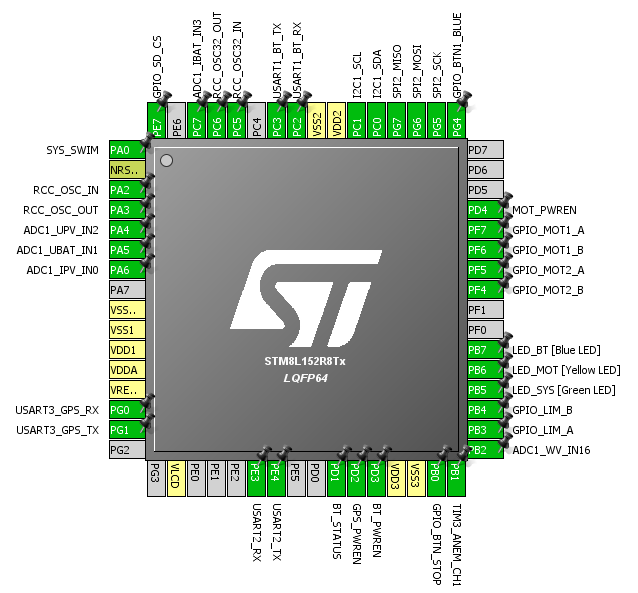
\includegraphics[width=.8\textwidth]{./img/stm8_pinout.PNG}
        \caption{Pin-Zuordnungen für den STM8-Mikrocontroller}
        \label{fig:mcu_pins}
    \end{figure}

    \begin{table}[H]
        \centering
        \begin{tabular}{|l|l|}
            \hline
            \textbf{Peripheral} & \textbf{Verwendung}                   \\
            \hline
            ADC1                & CPU-Temperatursensor,  Strom- und     \\
                                & Spannungssensoren, Richtungssignal    \\
                                & Windfahne                             \\
            GPIO                & Taster, LEDs, Endlagenschalter, Motor-\\
                                & treiber Steuersignale                 \\
            I2C                 & Digitale Sensoren                     \\
            SPI2                & SD-Karte                              \\
            TIM3                & Zähler für Anemometer-Geberimpulse    \\
            UART1               & UART-over-Bluetooth Umsetzer          \\
            UART2               & printf()-Debugausgaben                \\
            UART3               & NMEA 0183 Sentences vom GPS-Modul     \\
            \hline
        \end{tabular}
        \caption{Mikrocontroller-Peripheriemodule und ihr Einsatzzweck für die Wetterstation}
    \end{table}    

\section{Firmware}\label{cha:C-Code}
    Die entwickelte Mikrocontroller-Firmware definiert den Funktionsumfang der Wetterstation: neben der Auswertung und Aufzeichnung von Messdaten erfolgt die Ausrichtung des Solarpanels softwaregesteuert.
    
    Das Softwareprojekt ist dabei modular aufgebaut -- voneinander unabhängige Softwarekomponenten sind in eigene Module aufgeteilt. Funktionen zur Umrechnung der rohen Sensordaten in die gewünschten Darstellungen werden durch entsprechende Unterteilung in verschiedene Headerdateien vor anderen Teilen der Software ``versteckt''.
    
    Hieraus wurde eine die folgende Projektstruktur entwickelt:
    \begin{itemize}
        \item \texttt{main} -- Initialisierung des Systems beim Start und zyklische Datenverarbeitung im Hintergrund-Task
        \item \texttt{commlib/} -- Module zur Ansteuerung der seriellen Kommunikationsschnittstellen (UART, SPI, I\textsuperscript{2}C)
        \item \texttt{fslib/} -- Implementierung des FAT-Dateisystems für die SD-Karte, basierend auf der Open-Source Bibliothek ``FatFS''~\cite{elmchan_fatfs}
        \item \texttt{motorlib/} -- Motorsteuerung mit Reaktion auf Betätigung der Endlagenschalter in einer Interruptserviceroutine
        \item \texttt{powerlib/} -- C-Präprozessormakros für den Wechsel in den ``wait-for-interrupt'' Wartezustand
        \item \texttt{sensorlib/} -- Module zur Auswertung der digitalen und analogen Sensoren
        \item \texttt{stm8lib/} -- STM8 Standard Peripheral Library vom Mikrocontroller-Hersteller ST Microelectronics
        \item \texttt{userlib/} -- Module zur Steuerung des Systems auf einer höheren Abstraktionsebene
    \end{itemize}

    Die Software wurde dabei für eine interruptgesteuerte Verarbeitung ausgelegt. Der Mikrocontroller wird durch Timer-Interrupts in regelmäßigen Zeitabständen ``aufgeweckt'', um Steuerungsaufgaben auszuführen. Nach Abschluss der Ausführung wird er wieder in den Wartezustand ``wait-for-interrupt'' versetzt, um die Stromaufnahme während der Leerlaufzeit zu verringern.
    
    Nachfolgend wird auf einige der oben gelisteten Module näher eingegangen.
    
    \subsection{Auswertung der Sensoren (\texttt{sensorlib})}
    
        \subsubsection{BME280}\label{ssec:BME280}
            % Initialisierung
            % Sensordaten Typedef
    
        \subsubsection{CPU-Temperatursensor}
            % Auswertung über internen ADC-Kanal
            % Typedef

        \subsubsection{QMC5883L}\label{ssec:QMC5883L}
            % Initialisierung
            % Kalibrierung (Turm um 360° rotieren und X/Y Offset + Gain berechnen)
        
        \subsubsection{MPU6050}\label{ssec:MPU6050}
            % Initialisierung
            % Typedef
        
        \subsubsection{Anemometer und Windfahne}\label{ssec:Wind}
            % Anemometer: Drehgeber
            % Windfahne: ADC Kanal einlesen, Mapping über LUT, Kompassrichtung mit QMC5883
            
        \subsubsection{Strom- und Spannungsmessung}
            % ADC-Kanäle
            % Offset und Slope Bestimmung
       
    \subsection{GPS: NMEA 0183 Protokollverarbeitung}\label{ssec:GPS}
        % UART initialisierung
        % Einlesen: Start bei '$', Ende bei '\r'
        % LUT Sentence-Typen
        
    \subsection{Bluetooth: Aktivierung und AT-Befehlssatz}\label{ssec:AT_Commands}
        % BT-Modul deaktivieren, wenn längere Zeit nicht verbunden
        % siehe AT_Commands.md    
    
 